\documentclass{beamer}
\usetheme{default}

\usepackage{calc}
\usepackage{forloop}

\usepackage{xcolor}

\usepackage{tikz}

\usepackage{lstcustom}

\usepackage{tikz-uml}

% for footnotes

\usepackage[absolute,overlay]{textpos}

\newenvironment{reference}[2]{%
  \begin{textblock*}{\textwidth}(#1,#2)
      \footnotesize\it\bgroup\color{black!50!black}}{\egroup\end{textblock*}}

% End for footnotes

\title{Linked Lists}
\subtitle{Mark Royer}
\date{}


% Setup listing code styles

\lstdefinestyle{eclipseNoBox}{
  basicstyle={\small\lstfontfamily},
  emphstyle=\bfseries,
  keywordstyle=\color{keywordColor}\bfseries,
  commentstyle=\markupComments,
  stringstyle=\color{stringColor},
  numberstyle=\color{lineNumberColor}\lstfontfamily,
  morecomment=[s][\markupJavadocs]{/**}{*/}, % For Javadoc style comments
  showstringspaces=false,
  numbers=none,
}

\lstset{
  language=C++,
  style=eclipseNoBox,
  escapechar=\$
}

% End setup listing code styles



\usetikzlibrary{fit,calc,shadows,shapes.multipart,chains,arrows,snakes}


\begin{document}

%%%%%%%%%%%%%%%%%%%%%%%%%%%%%%%%%%%%%%%%%%%%%%%%%%%%%%%%%%%%

\begin{frame}
  \titlepage
\end{frame}

%%%%%%%%%%%%%%%%%%%%%%%%%%%%%%%%%%%%%%%%%%%%%%%%%%%%%%%%%%%%

\begin{frame}[t]{Linked lists}

~\\

\begin{itemize}
\item Arrays offer fast retrieval times due to the contiguous nature of the
data.

\item \textbf{Linked lists} store data in nodes, where each node
  contains the element and a pointer to the next one.

\item The first node is called the \textbf{head} and the last is the
  \textbf{tail}. 

\end{itemize}

~\\~\\

\begin{tikzpicture}[overlay,remember picture,list/.style={rectangle split, rectangle split parts=2,
     draw, rectangle split horizontal}, >=stealth, start chain,xshift=.5cm]
  %\draw[gray,step=0.25] (-1,-1) grid (1, 1);
  \node[list,on chain] (A) {$e_{0}$};
  \node[list,on chain] (B) {$e_{1}$};
  \node[on chain] (M) {...};
  \node[list,on chain] (C) {$e_{n-2}$};
  \node[list,on chain] (D) {$e_{n-1}$};
  \node[on chain,inner sep=0pt] (null) {\lstinline$NULL$};
  \node[] (head) [below=of A] {Head};
  \draw [->] (head.north) -- (A);
  \node[] (tail) [below=of D] {Tail};
  \draw [->] (tail.north) -- (D);
  \draw[*->] let \p1 = (A.two), \p2 = (A.center) in (\x1,\y2) -- (B);
  \draw[*->, decorate, decoration={snake,post length=1mm}] let \p1 = (B.two), \p2 = (B.center) in (\x1,\y2) -- (M);
  \draw [->, decorate, decoration={snake,post length=1mm}] (M.east) -- (C);
  \draw[*->] let \p1 = (C.two), \p2 = (C.center) in (\x1,\y2) -- (D);
  \draw[*->] let \p1 = (D.two), \p2 = (D.center) in (\x1,\y2) -- (null);
\end{tikzpicture}


\begin{reference}{4mm}{85mm}
  $n$ is the size of the list with $0 \dots n-1$ indices.
\end{reference} 

\end{frame}

%%%%%%%%%%%%%%%%%%%%%%%%%%%%%%%%%%%%%%%%%%%%%%%%%%%%%%%%%%%%

\begin{frame}[fragile]{Linked list advantages}

Advantages:

\begin{itemize}
\item Memory can be allocated and released as needed. Note arrays are
  sometimes oversized with many unused elements.
\item Some algorithms are faster than their array counterparts
\item Flexible nonlinear data structures can be created with nodes
  that utilize multiple pointers. Examples include the tree and the
  graph.
\end{itemize}

\pause

Disadvantages:

\begin{itemize}
\item Each node has the overhead of pointer fields.  At 4 bytes per
  pointer this can add up to more space than used for an array.
\item Some algorithms are slower than their array counterparts.
\end{itemize}


\end{frame}

%%%%%%%%%%%%%%%%%%%%%%%%%%%%%%%%%%%%%%%%%%%%%%%%%%%%%%%%%%%%


\begin{frame}[fragile]{The \lstinline$Node$ class}

Since the \lstinline$Node$ class is only used internally to the \lstinline$LinkedList$
  class, it is presented here with all public members.

~\\

\begin{lstlisting}[numbers=left]
template<typename T>
class Node {
public:
  Node() { next = NULL};
  Node(T element) {
    next = NULL;
    this->element = element;
  }

  T element;
  Node<T>* next;
};
\end{lstlisting}

\end{frame}

%%%%%%%%%%%%%%%%%%%%%%%%%%%%%%%%%%%%%%%%%%%%%%%%%%%%%%%%%%%%

\begin{frame}[fragile]{\lstinline$LinkedList$ initial insertion}

The \lstinline$LinkedList$ class has instance variables that point to
the head and tail. To insert three strings into an empty list:

\begin{enumerate}
\item Create the the first node and insert into the list.

\begin{lstlisting}
head = new Node<string>("Chicago");
tail = head;
\end{lstlisting}

\pause

\item Create the second node and insert it into the list.

\begin{lstlisting}
tail->next = new Node<string>("Dallas");
tail = tail->next;
\end{lstlisting}

\pause

\item Create the third node and insert it to the list.

\begin{lstlisting}
tail->next = new Node<string>("Denver");
tail = tail->next;
\end{lstlisting}

\end{enumerate}

\end{frame}

%%%%%%%%%%%%%%%%%%%%%%%%%%%%%%%%%%%%%%%%%%%%%%%%%%%%%%%%%%%%

\begin{frame}[fragile]{List traversal}

\begin{itemize}

\item Lists can only be traveled from the head node to the tail node. Unlike
arrays there is no direct access to any particular element. This is
the primary disadvantage of a list.

\item Given a \lstinline$Node$, the following display function outputs the elements.

\begin{lstlisting}
void display (Node<string>* head) {
  Node<string>* current = head;
  while (current != NULL) {
    cout << current->element << " ";
    current = current->next;
  }
}
\end{lstlisting}

\end{itemize}

\end{frame}

%%%%%%%%%%%%%%%%%%%%%%%%%%%%%%%%%%%%%%%%%%%%%%%%%%%%%%%%%%%%

\begin{frame}[fragile]{\lstinline$LinkedList$ class}

\begin{tikzpicture}
\umlclass[template=T]{LinkedList}
% fields
{
-head: Node<T>*\\
-tail: Node<T>* \\
-size: int 
}
% methods
{
+LinkedList() \\
+addFirst(element: T): void \\
+addLast(element: T): void \\ 
+add(index: int, element: T): void \\ 
+removeFirst(): T \\
+removeLast(): T \\
+removeAt(index: int): T \\
+set(index: int, element: T): T \\
- Additional methods omitted -
}%


\end{tikzpicture}

\end{frame}

%%%%%%%%%%%%%%%%%%%%%%%%%%%%%%%%%%%%%%%%%%%%%%%%%%%%%%%%%%%%

\begin{frame}[fragile]{LinkedList.h}

\begin{itemize}

\item The LinkedList template class is completely contained within
  file LinkedList.h.

\item The general contents of LinkedList.h is

\end{itemize}

\begin{lstlisting}[frame=tblr]
// File: LinkedList.h

// Code for template class Node

// Class definition for template class LinkedList

// Implementation of functions for template class
// LinkedList
\end{lstlisting}



\end{frame}

%%%%%%%%%%%%%%%%%%%%%%%%%%%%%%%%%%%%%%%%%%%%%%%%%%%%%%%%%%%%

\begin{frame}[fragile]{\lstinline$LinkedList$ definition}

\begin{itemize}
\item Private data includes pointers to head and tail and an integer
  node count.

\item Notice how a pointer to template Node object is declared.

\item The unknown type T is used in the declaration.

\item T will not be known until the template is given a type for T.

\end{itemize}

\begin{lstlisting}
template<typename T>
class LinkedList {
public:
  // constructors and functions
private:
  Node<T>* head;
  Node<T>* tail;
  int size;
};
\end{lstlisting}

\end{frame}

%%%%%%%%%%%%%%%%%%%%%%%%%%%%%%%%%%%%%%%%%%%%%%%%%%%%%%%%%%%%

\begin{frame}[fragile]{Default constructor}

\begin{itemize}
\item Only one default constructor can be defined.

\item The default constructor for a \lstinline$LinkedList$ creates an empty list.
\end{itemize}

\begin{lstlisting}[numbers=left]
template <typename T>
LinkedList<T>::LinkedList() {
  head = NULL;
  tail = NULL:
  size = 0;
}
\end{lstlisting}

\end{frame}

%%%%%%%%%%%%%%%%%%%%%%%%%%%%%%%%%%%%%%%%%%%%%%%%%%%%%%%%%%%%

\begin{frame}[fragile]{Adding elements}

\begin{itemize}
\item Elements can be added to the beginning of the list, the end of
  the list, or at an internal position.

\item When writing linked list algorithms, any case that modifies the
  head or tail pointers must be treated as a special case. When
  testing code, ask the following questions:

  \begin{enumerate}

  \item Does the code work on an empty list?

  \item Does the code work on a list where head and/or tail might
    change?
      
  \item Does the code work on an internal node in a list of multiple
    items?

  \end{enumerate}

\end{itemize}

\end{frame}

%%%%%%%%%%%%%%%%%%%%%%%%%%%%%%%%%%%%%%%%%%%%%%%%%%%%%%%%%%%%

\begin{frame}[fragile]{The \lstinline$addFirst$ method }

\begin{itemize}
\item Adds a new item at the beginning
of a list.

\item  In all cases, the head pointer will
change. 

\item On an empty list, the tail pointer will
also change.

\end{itemize}

\begin{lstlisting}[numbers=left]
template<typename T>
void LinkedList<T>::addFirst(T element) {
  Node<T>* newNode = new Node<T>(element);
  newNode->next = head;
  head = newNode;
  size++;
  if (tail == NULL)
    tail = head;
}
\end{lstlisting}



\end{frame}

%%%%%%%%%%%%%%%%%%%%%%%%%%%%%%%%%%%%%%%%%%%%%%%%%%%%%%%%%%%%


\begin{frame}[fragile,t]{The \lstinline$addFirst$ method }

\only<1,2> {Before the new node is inserted. The new node is shown in \textcolor{blue}{blue}.}

\only<3> {After the new node is inserted.}

~\\~\\~\\~\\

\begin{tikzpicture}[overlay,remember picture,list/.style={rectangle split, rectangle split parts=2,
     draw, rectangle split horizontal, node distance=.5cm}, >=stealth, start chain,xshift=.5cm]
  %\draw[gray,step=0.25] (-1,-1) grid (1, 1);
  \node<3>[list,on chain, color=blue] (newone) {$x_{}$};
  \node[list,on chain] (A) {$e_{0}$};
  \node[list,on chain] (B) {$e_{1}$};
  \node[on chain] (M) {...};
  \node[list,on chain] (C) {$e_{n-2}$};
  \node[list,on chain] (D) {$e_{n-1}$};
  \node[on chain,inner sep=0pt] (null) {\lstinline$NULL$};
  \node<1,2>[] (head) [below=of A] {Head};
  \node<3>[] (head) [below=of newone] {Head};
  \node<1,2>[list, above right of=A, above=1cm,color=blue] (newone) {$x_{}$};
  \path<2>[black, line width=2pt, ->] (newone.west) edge [out=180, in=180] (A.west);
  \draw<1,2>[->] (head.north) -- (A);
  \draw<3>[->] (head.north) -- (newone);
  \node[] (tail) [below=of D] {Tail};
  \draw [->] (tail.north) -- (D);
  \draw<3>[*->] let \p1 = (newone.two), \p2 = (newone.center) in (\x1,\y2) -- (A);
  \draw[*->] let \p1 = (A.two), \p2 = (A.center) in (\x1,\y2) -- (B);
  \draw[*->, decorate, decoration={snake,post length=1mm}] let \p1 = (B.two), \p2 = (B.center) in (\x1,\y2) -- (M);
  \draw [->, decorate, decoration={snake,post length=1mm}] (M.east) -- (C);
  \draw[*->] let \p1 = (C.two), \p2 = (C.center) in (\x1,\y2) -- (D);
  \draw[*->] let \p1 = (D.two), \p2 = (D.center) in (\x1,\y2) -- (null);
\end{tikzpicture}

\begin{reference}{4mm}{85mm}
  $n$ is the size of the list prior to insertion with $0 \dots n-1$ indices.
\end{reference} 

\end{frame}

%%%%%%%%%%%%%%%%%%%%%%%%%%%%%%%%%%%%%%%%%%%%%%%%%%%%%%%%%%%%


\begin{frame}[fragile]{The \lstinline$addLast$ method }

\begin{itemize}
\item This function adds a new item at the end of a
list. 

\item In all cases, the tail pointer will change.

\item On an empty list, the head pointer will also
change.

\end{itemize}

\begin{lstlisting}[numbers=left]
template<typename T>
void LinkedList<T>::addLast(T element) {
  Node<T> *newNode = new Node<T>(element);
  if (tail == NULL)
    head = tail = newNode;
  else {
    tail->next = newNode;
    tail = tail->next;
  }
  size++;
}
\end{lstlisting}

\end{frame}

%%%%%%%%%%%%%%%%%%%%%%%%%%%%%%%%%%%%%%%%%%%%%%%%%%%%%%%%%%%%


\begin{frame}[fragile,t]{The \lstinline$addLast$ method }

\only<1,2> {Before the new node is inserted. The new node is shown in \textcolor{blue}{blue}.}

\only<3> {After the new node is inserted.}

~\\~\\~\\~\\

\begin{tikzpicture}[overlay,remember picture,list/.style={rectangle split, rectangle split parts=2,
     draw, rectangle split horizontal, node distance=.5cm}, >=stealth, start chain,xshift=.5cm]
  %\draw[gray,step=0.25] (-1,-1) grid (1, 1);
  \node[list,on chain] (A) {$e_{0}$};
  \node[list,on chain] (B) {$e_{1}$};
  \node[on chain] (M) {...};
  \node[list,on chain] (C) {$e_{n-2}$};
  \node[list,on chain] (D) {$e_{n-1}$};
  \node<3>[list,on chain, color=blue] (newone) {$x_{}$};
  \node[on chain,inner sep=0pt] (null) {\lstinline$NULL$};
  \node[] (head) [below=of A] {Head};
  \node<1,2>[list, above left of=D, above=1cm,color=blue] (newone) {$x_{}$};
  \path<2>[black, line width=2pt, ->] (newone.east) edge [out=0, in=45] (D.north east);
  \draw[->] (head.north) -- (A);
  \node<1,2>[] (tail) [below=of D] {Tail};
  \node<3>[] (tail) [below=of newone] {Tail};
  \draw<1,2>[->] (tail.north) -- (D);
  \draw<3>[->] (tail.north) -- (newone);
  \draw[*->] let \p1 = (A.two), \p2 = (A.center) in (\x1,\y2) -- (B);
  \draw[*->, decorate, decoration={snake,post length=1mm}] let \p1 = (B.two), \p2 = (B.center) in (\x1,\y2) -- (M);
  \draw [->, decorate, decoration={snake,post length=1mm}] (M.east) -- (C);
  \draw[*->] let \p1 = (C.two), \p2 = (C.center) in (\x1,\y2) -- (D);
  \draw<1,2>[*->] let \p1 = (D.two), \p2 = (D.center) in (\x1,\y2) -- (null);
  \draw<3>[*->] let \p1 = (D.two), \p2 = (D.center) in (\x1,\y2) -- (newone);
  \draw<3>[*->] let \p1 = (newone.two), \p2 = (newone.center) in (\x1,\y2) -- (null);
\end{tikzpicture}

\begin{reference}{4mm}{85mm}
  $n$ is the size of the list prior to insertion with $0 \dots n-1$ indices.
\end{reference} 

\end{frame}

%%%%%%%%%%%%%%%%%%%%%%%%%%%%%%%%%%%%%%%%%%%%%%%%%%%%%%%%%%%%

\begin{frame}[fragile]{The \lstinline$add$ method }

\begin{itemize}
\item If the index is 0, a call is made to the addFirst function.
\item If the index is size-1, a call is made to the addLast function.
\item Otherwise traverse the list sequentially and find the location to insert.
\end{itemize}

\begin{lstlisting}
template<typename T>
void LinkedList<T>::add(int index, T element) {
  if (index == 0)
    addFirst(element);
  else if (index >= size)
    addLast(element);
  else {
    // Code on next slide
  }
}
\end{lstlisting}

\end{frame}

%%%%%%%%%%%%%%%%%%%%%%%%%%%%%%%%%%%%%%%%%%%%%%%%%%%%%%%%%%%%

\begin{frame}[fragile]{The \lstinline$add$ method traversal}

The algorithm needs to traverse the
list sequentially, maintaining pointers to the
node at and after the insertion point. Once the
position is located, a new node is created and
the pointers are adjusted.

\begin{lstlisting}
  // contents of final else
  Node<T>* current = head;
  for (int i = 1; i < index; i++)
    current = current->next;
  Node<T>* temp = current->next;
  current->next = new Node<T>(element);
  current->next->next = temp;
  size++;
\end{lstlisting}

\end{frame}

%%%%%%%%%%%%%%%%%%%%%%%%%%%%%%%%%%%%%%%%%%%%%%%%%%%%%%%%%%%%

\begin{frame}[fragile,t]{The \lstinline$add$ method }

\only<1,2> {Before the new node is inserted at position $i$. The new node is shown in \textcolor{blue}{blue}.}

\only<3> {After the new node is inserted.\\~\\}

~\\~\\~\\~\\

\begin{tikzpicture}[overlay,remember picture,list/.style={rectangle split, rectangle split parts=2,
     draw, rectangle split horizontal, node distance=.3cm}, >=stealth, start chain]
  %\draw[gray,step=0.25] (-1,-1) grid (1, 1);
  \node[list,on chain] (A) {$e_{0}$};
  \node[on chain] (J) {...};
  \node[list,on chain] (B) {$e_{i-1}$};
  \node<3>[list,on chain, color=blue] (newone) {$x_{}$};
  \node[list,on chain] (C) {\only<1,2>{$e_{i}$}\only<3>{$e_{i+1}$}};
  \node[on chain] (M) {...};
  \node[list,on chain] (D) {$e_{n-1}$};
  \node[on chain,inner sep=0pt] (null) {\lstinline$NULL$};
  \node[] (head) [below=of A] {Head};
  \node<1,2>[list, above left of=C, above=1cm,color=blue] (newone) {$x_{}$};
  \path<2>[black, line width=2pt, ->] (newone.south) edge [out=270, in=45] (B.north east);
  \draw[->] (head.north) -- (A);
  \node[] (tail) [below=of D] {Tail};
  \draw[->] (tail.north) -- (D);
  \draw[*->, decorate, decoration={snake,post length=1mm}] let \p1 = (A.two), \p2 = (A.center) in (\x1,\y2) -- (J);
  \draw[->, decorate, decoration={snake,post length=1mm}] (J.east) -- (B);
  \draw<1,2>[*->] let \p1 = (B.two), \p2 = (B.center) in (\x1,\y2) -- (C);
  \draw<3>[*->] let \p1 = (B.two), \p2 = (B.center) in (\x1,\y2) -- (newone);
  \draw<3>[*->] let \p1 = (newone.two), \p2 = (newone.center) in (\x1,\y2) -- (C);
  \draw[*->, decorate, decoration={snake,post length=1mm}] let \p1 = (C.two), \p2 = (C.center) in (\x1,\y2) -- (M);
  \draw[->, decorate, decoration={snake,post length=1mm}] (M.east) -- (D);
  \draw[*->] let \p1 = (D.two), \p2 = (D.center) in (\x1,\y2) -- (null);
\end{tikzpicture}

\begin{reference}{4mm}{85mm}
  $n$ is the size of the list prior to insertion with $0 \dots n-1$ indices.
\end{reference} 

\end{frame}

%%%%%%%%%%%%%%%%%%%%%%%%%%%%%%%%%%%%%%%%%%%%%%%%%%%%%%%%%%%%



\begin{frame}[fragile]{Removing elements}

In the list, elements can be removed from:

\begin{itemize}
\item The beginning of the list
\item The end of the list
\item An internal position
\end{itemize}

\end{frame}

%%%%%%%%%%%%%%%%%%%%%%%%%%%%%%%%%%%%%%%%%%%%%%%%%%%%%%%%%%%%

\begin{frame}[fragile]{The \lstinline$removeFirst$ method}

\begin{itemize}
\item Removes the item from the beginning of a list and returns its
  value to the user.

\item In all cases, the head pointer will change.

\item On a list of one item, the tail pointer will also change. A PRE
  condition states that the list is not empty.
\end{itemize}

\begin{lstlisting}[numbers=left]
template<typename T>
T LinkedList<T>::removeFirst() {
  Node<T>* temp = head;
  head = head->next;
  size--;
  if (head == NULL)
    tail = NULL;
  T element = temp->element;
  delete temp;
  return element;
}
\end{lstlisting}

\end{frame}

%%%%%%%%%%%%%%%%%%%%%%%%%%%%%%%%%%%%%%%%%%%%%%%%%%%%%%%%%%%%

\begin{frame}[fragile,t]{The \lstinline$removeFirst$ method }

\only<1> {Before the node is deleted.}

\only<2> {After the node is deleted.}

~\\~\\~\\~\\

\begin{tikzpicture}[overlay,remember picture,list/.style={rectangle split, rectangle split parts=2,
     draw, rectangle split horizontal, node distance=.5cm}, >=stealth, start chain,xshift=.5cm]
  %\draw[gray,step=0.25] (-1,-1) grid (1, 1);
  \node<1>[list,on chain, color=blue] (A) {$e_{0}$};
  \node[list,on chain] (B) {$e_{1}$};
  \node[on chain] (M) {...};
  \node[list,on chain] (C) {$e_{n-2}$};
  \node[list,on chain] (D) {$e_{n-1}$};
  \node[on chain,inner sep=0pt] (null) {\lstinline$NULL$};
  \node<1>[] (head) [below=of A] {Head};
  \node<2>[] (head) [below=of B] {Head};
  \node<1>[above right of=A, above right=1cm,color=blue] (newone) {Node to delete};
  \path<1>[black, line width=2pt, ->] (newone.west) edge [out=180, in=90] (A.north);
  \draw<1>[->] (head.north) -- (A);
  \draw<2>[->] (head.north) -- (B);
  \node[] (tail) [below=of D] {Tail};
  \draw [->] (tail.north) -- (D);
  \draw<1>[*->] let \p1 = (A.two), \p2 = (A.center) in (\x1,\y2) -- (B);
  \draw[*->, decorate, decoration={snake,post length=1mm}] let \p1 = (B.two), \p2 = (B.center) in (\x1,\y2) -- (M);
  \draw [->, decorate, decoration={snake,post length=1mm}] (M.east) -- (C);
  \draw[*->] let \p1 = (C.two), \p2 = (C.center) in (\x1,\y2) -- (D);
  \draw[*->] let \p1 = (D.two), \p2 = (D.center) in (\x1,\y2) -- (null);
\end{tikzpicture}

\begin{reference}{4mm}{85mm}
  $n$ is the size of the list prior to deletion with $0 \dots n-1$ indices.
\end{reference} 

\end{frame}

%%%%%%%%%%%%%%%%%%%%%%%%%%%%%%%%%%%%%%%%%%%%%%%%%%%%%%%%%%%%

\begin{frame}[fragile]{The \lstinline$removeLast$ method}

\begin{itemize}
\item This function removes the item from the end of a list and
  returns its value to the user.
\item In all cases, the tail pointer will change.
\item On a list one item, the head pointer will also change.
\item A precondition states that the list is not empty. Since there
  is no direct access to the node just prior to the tail node, a list
  traversal must take place.
\end{itemize}

\end{frame}

%%%%%%%%%%%%%%%%%%%%%%%%%%%%%%%%%%%%%%%%%%%%%%%%%%%%%%%%%%%%

\begin{frame}[fragile]{The \lstinline$removeLast$ method}

\begin{lstlisting}[numbers=left]
template<typename T>
T LinkedList<T>::removeLast() {
  Node<T>* temp = tail;
  if (size == 1)
    head = tail = NULL;
  else {
    Node<t>* current = head;
    for (int i = 0; i < size - 2; i++)
      current = current->next;
    tail = current;
    tail->next = NULL;
  }
  size--;
  T element = temp->element;
  delete temp;
  return element;
}
\end{lstlisting}

\end{frame}

%%%%%%%%%%%%%%%%%%%%%%%%%%%%%%%%%%%%%%%%%%%%%%%%%%%%%%%%%%%%

\begin{frame}[fragile,t]{The \lstinline$removeLast$ method }

\only<1> {Before the last node is deleted.}

\only<2> {After the node is deleted.}

~\\~\\~\\~\\

\begin{tikzpicture}[overlay,remember picture,list/.style={rectangle split, rectangle split parts=2,
     draw, rectangle split horizontal}, >=stealth, start chain,xshift=.5cm]
  %\draw[gray,step=0.25] (-1,-1) grid (1, 1);
  \node[list,on chain] (A) {$e_{0}$};
  \node[list,on chain] (B) {$e_{1}$};
  \node[on chain] (M) {...};
  \node[list,on chain] (C) {$e_{n-2}$};
  \node<1>[list,on chain, color=blue] (D) {$e_{n-1}$};
  \node[on chain,inner sep=0pt] (null) {\lstinline$NULL$};
  \node[] (head) [below=of A] {Head};
  \node<1>[above left of=D, above left=1cm, color=blue] (newone) {Node to delete};
  \path<1>[black, line width=2pt, ->] (newone.east) edge [out=0, in=90] (D.north);
  \draw[->] (head.north) -- (A);
  \node<1>[] (tail) [below=of D] {Tail};
  \node<2>[] (tail) [below=of C] {Tail};
  \draw<1>[->] (tail.north) -- (D);
  \draw<2>[->] (tail.north) -- (C);
  \draw[*->] let \p1 = (A.two), \p2 = (A.center) in (\x1,\y2) -- (B);
  \draw[*->, decorate, decoration={snake,post length=1mm}] let \p1 = (B.two), \p2 = (B.center) in (\x1,\y2) -- (M);
  \draw [->, decorate, decoration={snake,post length=1mm}] (M.east) -- (C);
  \draw<1>[*->] let \p1 = (C.two), \p2 = (C.center) in (\x1,\y2) -- (D);
  \draw<2>[*->] let \p1 = (C.two), \p2 = (C.center) in (\x1,\y2) -- (null);
  \draw<1>[*->] let \p1 = (D.two), \p2 = (D.center) in (\x1,\y2) -- (null);
\end{tikzpicture}

\begin{reference}{4mm}{85mm}
  $n$ is the size of the list prior to deletion with $0 \dots n-1$ indices.
\end{reference} 

\end{frame}

%%%%%%%%%%%%%%%%%%%%%%%%%%%%%%%%%%%%%%%%%%%%%%%%%%%%%%%%%%%%

\begin{frame}[fragile]{The \lstinline$removeAt$ method}

\begin{itemize}
\item If the index is 0, a call is made to the
removeFirst function.
\item If the index is >= size, a call is made to the
removeLast function.
\item Otherwise it is known to be an internal removal. Traverse the
  list sequentially, maintaining pointers to the node right before the
  removal point. Once the position is located, the node is taken out
  and the pointers are adjusted.
\end{itemize}

\end{frame}

%%%%%%%%%%%%%%%%%%%%%%%%%%%%%%%%%%%%%%%%%%%%%%%%%%%%%%%%%%%%

\begin{frame}[fragile]{The \lstinline$removeAt$ method}

The final else statement contains the following code:

\begin{lstlisting}[numbers=left]
Node<T>* previous = head; 

for (int i = 1; i < index; i++)
  previous = previous->next;

// current points to removal position
Node<T>* current = previous->next; 
previous->next = current->next;    // adjust pointers

size--;
T element = current->element;      // save item from current
delete current;	                   // delete current
return element;
\end{lstlisting}

\end{frame}

%%%%%%%%%%%%%%%%%%%%%%%%%%%%%%%%%%%%%%%%%%%%%%%%%%%%%%%%%%%%

\begin{frame}[fragile,t]{The \lstinline$removeAt$ method }

\only<1> {Before the node is deleted at position $i$.}

\only<2> {After the node is deleted.}

~\\~\\~\\~\\

\begin{tikzpicture}[overlay,remember picture,list/.style={rectangle split, rectangle split parts=2,
     draw, rectangle split horizontal, node distance=.3cm}, >=stealth, start chain]
  %\draw[gray,step=0.25] (-1,-1) grid (1, 1);
  \node[list,on chain] (A) {$e_{0}$};
  \node[on chain] (J) {...};
  \node[list,on chain] (B) {$e_{i-1}$};
  \node<1>[list,on chain, color=blue] (C) {\only<1,2>{$e_{i}$}\only<3>{$e_{i+1}$}};
  \node[list,on chain] (D) {$e_{i+1}$};
  \node[on chain] (M) {...};
  \node[list,on chain] (E) {$e_{n-1}$};
  \node[on chain,inner sep=0pt] (null) {\lstinline$NULL$};
  \node[] (head) [below=of A] {Head};
  \node<1>[above of=C, above=.5cm,color=blue] (comment) {Node to delete};
 
  \node[below left of=B,below=.4cm] (previous) {previous};
  \draw[->] (previous.north) -- (B);
  \node<1>[below of=C,below =.4cm] (current) {current};
  \draw<1>[->] (current.north) -- (C);
  \node[below right of=D,below=.4cm] (currentnext) {\lstinline$current->next$};
  \draw[->] (currentnext.north) -- (D);

  \path<1>[black, line width=2pt, ->] (comment.south) edge [out=270, in=90] (C.north);
  \draw[->] (head.north) -- (A);
  \node[] (tail) [below=of E] {Tail};
  \draw[->] (tail.north) -- (E);
  \draw[*->, decorate, decoration={snake,post length=1mm}] let \p1 = (A.two), \p2 = (A.center) in (\x1,\y2) -- (J);
  \draw[->, decorate, decoration={snake,post length=1mm}] (J.east) -- (B);
  \draw<1>[*->] let \p1 = (B.two), \p2 = (B.center) in (\x1,\y2) -- (C);
  \draw<2>[*->] let \p1 = (B.two), \p2 = (B.center) in (\x1,\y2) -- (D);
  \draw<1>[*->] let \p1 = (C.two), \p2 = (C.center) in (\x1,\y2) -- (D);
  \draw[*->, decorate, decoration={snake,post length=1mm}] let \p1 = (D.two), \p2 = (D.center) in (\x1,\y2) -- (M);
  \draw[->, decorate, decoration={snake,post length=1mm}] (M.east) -- (E);
  \draw[*->] let \p1 = (E.two), \p2 = (E.center) in (\x1,\y2) -- (null);
\end{tikzpicture}

\begin{reference}{4mm}{85mm}
  $n$ is the size of the list prior to deletion with $0 \dots n-1$ indices.
\end{reference} 

\end{frame}

%%%%%%%%%%%%%%%%%%%%%%%%%%%%%%%%%%%%%%%%%%%%%%%%%%%%%%%%%%%%

\begin{frame}[fragile]{Rule of three}

The rule of three states that if you create one of the following: 

~\\

\begin{description}

\item[Destructor\ \ \ \ ] \hfill \\ % Not sure why I need padding

\lstinline$Type::~Type()$

\item[Copy constructor] \hfill \\

\lstinline$Type::Type(const Type& other)$

\item[Assignment operator] \hfill \\

\lstinline$Type& Type::operator=(const Type& other)$

\end{description}

~\\

Then you probably want to explicitly define all three.

\end{frame}

%%%%%%%%%%%%%%%%%%%%%%%%%%%%%%%%%%%%%%%%%%%%%%%%%%%%%%%%%%%%

\begin{frame}[fragile]{Rule of three examples}

Common tasks using objects:

~\\

\begin{lstlisting}[numbers=left]
LinkedList<int> one;          // Default constructor

LinkedList<int> two(one);     // Copy constructor

LinkedList<int> three = two;  // Copy constructor

three = one;                  // assignment

// Objects destructed automatically on the run-time stack
\end{lstlisting}

\end{frame}

%%%%%%%%%%%%%%%%%%%%%%%%%%%%%%%%%%%%%%%%%%%%%%%%%%%%%%%%%%%%

\begin{frame}[fragile]{Destructor}

The destructor function must traverse the list deallocating each node.

\begin{lstlisting}[numbers=left]
template<typename T>
LinkedList<T>::~LinkedList() {
  Node<T>* current = head; // current advances through list
  Node<T>* temp = current; // temp points to node to be deleted

  while (current != NULL) {
    current = current -> next;
    delete temp;
    temp = current;
  }
}
\end{lstlisting}

\end{frame}

%%%%%%%%%%%%%%%%%%%%%%%%%%%%%%%%%%%%%%%%%%%%%%%%%%%%%%%%%%%%

\begin{frame}[fragile]{Copy constructor}

The copy constructor is called when a new object is constructed from
an existing one.  A traversal of the other list copies nodes one at a
time to the object.

\begin{lstlisting}[numbers=left]
template<typename T>
LinkedList<T>::LinkedList (LinkedList<T>& other ) {
  head = tail = NULL;
  size = 0;

  Node<T>* current = other.head;
  while (current != NULL) {
    addLast (current->element);
    current = current->next;
  }
}
\end{lstlisting}

\end{frame}

%%%%%%%%%%%%%%%%%%%%%%%%%%%%%%%%%%%%%%%%%%%%%%%%%%%%%%%%%%%%

\begin{frame}[fragile]{Assignment operator}

\begin{itemize}

\item Delete the current list and then copy the other list.

\item Note, the object destructor function is called.

\item Note, the use of \lstinline$this$ syntax.

\end{itemize}

\begin{lstlisting}[numbers=left]
LinkedList<T>& LinkedList<T>::operator=(
                      const LinkedList<T>& other) {
  if (&other == this) 
    return *this;               // case of self-assignment
  LinkedList<T>::~LinkedList();
  Node<T>* current = other.head;
  head = tail = NULL;
  size = 0;
  while (current != NULL) {
    addLast (current->element); // add node to end of object
    current = current->next;
  }
  return *this;
}
\end{lstlisting}

\end{frame}

%%%%%%%%%%%%%%%%%%%%%%%%%%%%%%%%%%%%%%%%%%%%%%%%%%%%%%%%%%%%





\end{document}

%  LocalWords:  xshift sep oversized LinkedList typename cout addLast
%  LocalWords:  addFirst removeFirst removeLast removeAt newNode PRE
%  LocalWords:  newone currentnext const
